%----------------------------------------------------------------
%
%  File    :  thesis-tech.tex
%
%  Author  :  Eva Rott, TU Graz, Austria
% 
%  Created :  14 May 2017
% 
%  Changed :  16 May 2017
% 
%----------------------------------------------------------------


\chapter{Matrix Headers}
\label{chap:headers}

A standard matrix visualization contains a symmetric grid representing the node connections and node labels on top and to the left side of the grid. In this survey this area and in general the area around the grid is referred to as matrix header. The matrix header can be used for visualizing additional information about the matrix data. An example for that is a group of node connections, the node density or the current level of zoom in a multi-layer matrix.
There are various techniques to achieve additional information visualization in a matrix header. Most of them can be found in the program Matrix Explorer.

The Matrix Explorer is another tool for matrix visualization of graphs. As seen in figure \ref{fig:header_matrixexplorer}, the program displays the matrix without a zoom functionality, while giving a small overview of the full matrix in the top left corner of the graphical user interface. Aside from the matrix visualization, the Matrix Explorer provides various options for filtering and sorting of nodes and executing operations on the matrix headers. The following section describes the most common operations and gives one example per listed header visualization technique for a better understanding. 

\begin{figure}[tp]
  \centering
  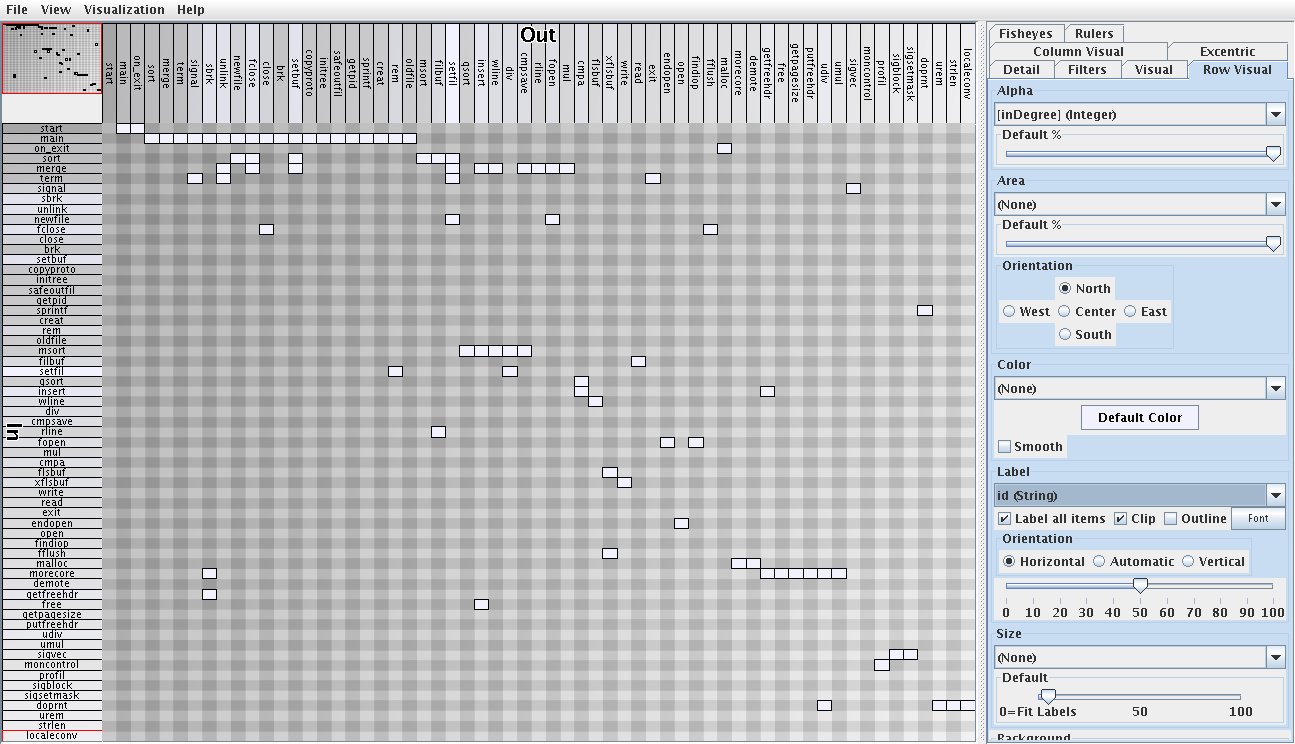
\includegraphics[keepaspectratio,width=\hsize,height=\halfh]
  {images/Header_MatrixExplorer.png}
  
  \caption[Matrix Visualization Tool Matrix Explorer]{
  The graphical user interface of the matrix visualization tool Matrix Explorer \citep{henry-phd-2008}.
  \imgcredit{Screenshot created by an author of this thesis using Matrix Explorer. \citep{henry-phd-2008}.}
  }
  \label{fig:header_matrixexplorer}
\end{figure}

\section{Node Connections}
As seen in figure \ref{fig:header_matlink} from the program MatLink, created by \citep[105-118]{henry-phd-2008} curved lines are used for highlighting node connections. The shortest path is highlighted in red. When one node is selected, the program draws the paths in the headers of the matrix. Using this visual information it can quickly be seen how many other nodes are connected directly to the selected node. In addition, the path from one node to another connected node can be traversed using these lines \citep[105-118]{henry-phd-2008}.

\begin{figure}[tp]
  \centering
  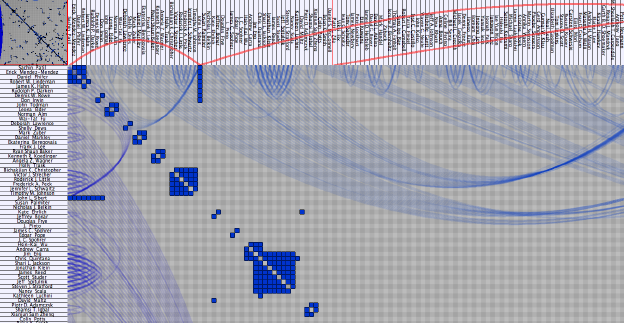
\includegraphics[keepaspectratio,width=\hsize,height=\halfh]
  {images/Header_MatLink_path.png}
  
  \caption[Highlighting Matrix Paths]{
  In the program MatLink \citep[105-118]{henry-phd-2008} the paths between selected nodes are highlighted using curved lines. The shortest path is drawn in red.
  \imgcredit{Image taken from the master thesis \citep[105-118]{henry-phd-2008}.}
  }
  \label{fig:header_matlink}
\end{figure}

\section{Histogram per Node}
\label{sec:histogram-per-node}
A histogram can be computed over various node properties. An example for such a property is the node degree. The Matrix Explorer offers this histogram functionality. Figure \ref{fig:header_matrixexplorer_histogram} shows a matrix visualization of data similar to that used for the first two examples in the previous chapter. Again, a set of functions from a program are represented as nodes and the programs control flow as links. Looking at the histogram which was computed over the outgoing links it becomes obvious that the main function has the largest light gray area. This means that it has the largest number of outgoing links of all nodes. In contrast to the node out degree distribution, the incoming links follow a more balanced distribution. Considering this example, a histogram in the header is well suited for showing the general distribution of the node degree. In case nodes containing extreme values should be highlighted, the header color visualization technique can be used.

\begin{figure}[tp]
  \centering
  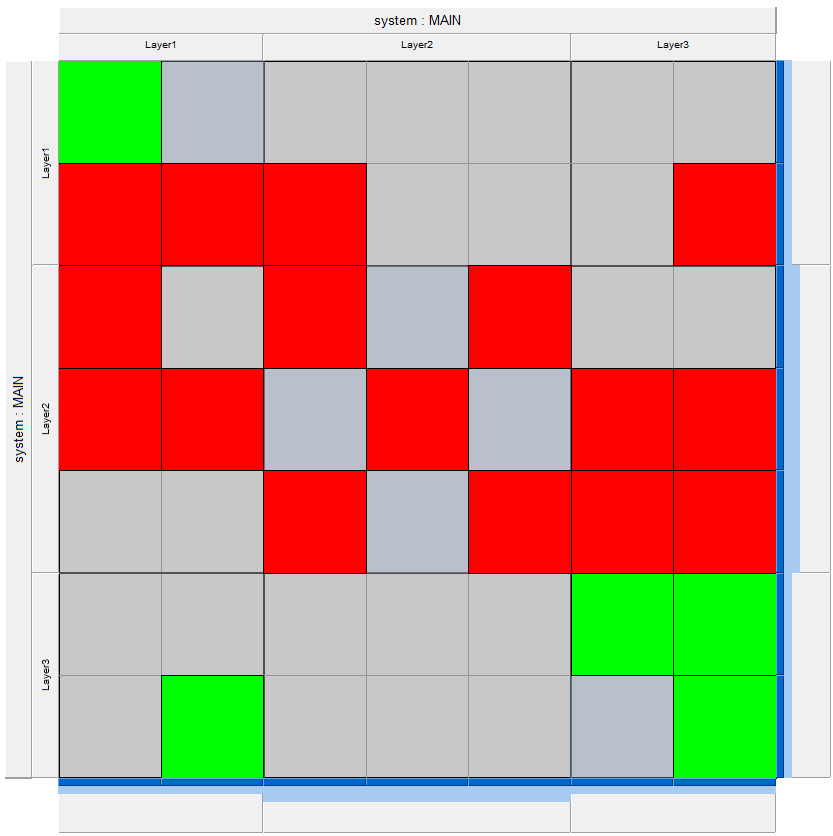
\includegraphics[keepaspectratio,width=\hsize,height=\halfh]
  {images/Header_MatrixExplorer_histogram.png}
  
  \caption[Matrix Header with Histogram of Node Degree]{
  The size of the white area in the node label represents the node degree.
  \imgcredit{Screenshot created by an author of this thesis using Matrix Explorer. \citep{henry-phd-2008}.}
  }
  \label{fig:header_matrixexplorer_histogram}
\end{figure}

\section{Color Highlighting}
Every node in a graph can be assigned a color in a certain range. This color distribution assigned to the nodes can be computed for the same properties as the histogram. The darker the color the higher the value of this node. Considering the same example and figure \ref{fig:header_matrixexplorer_color} as in the previous section, it becomes obvious that the start function has no incoming links as it is the root function of the program.

\begin{figure}[tp]
  \centering
  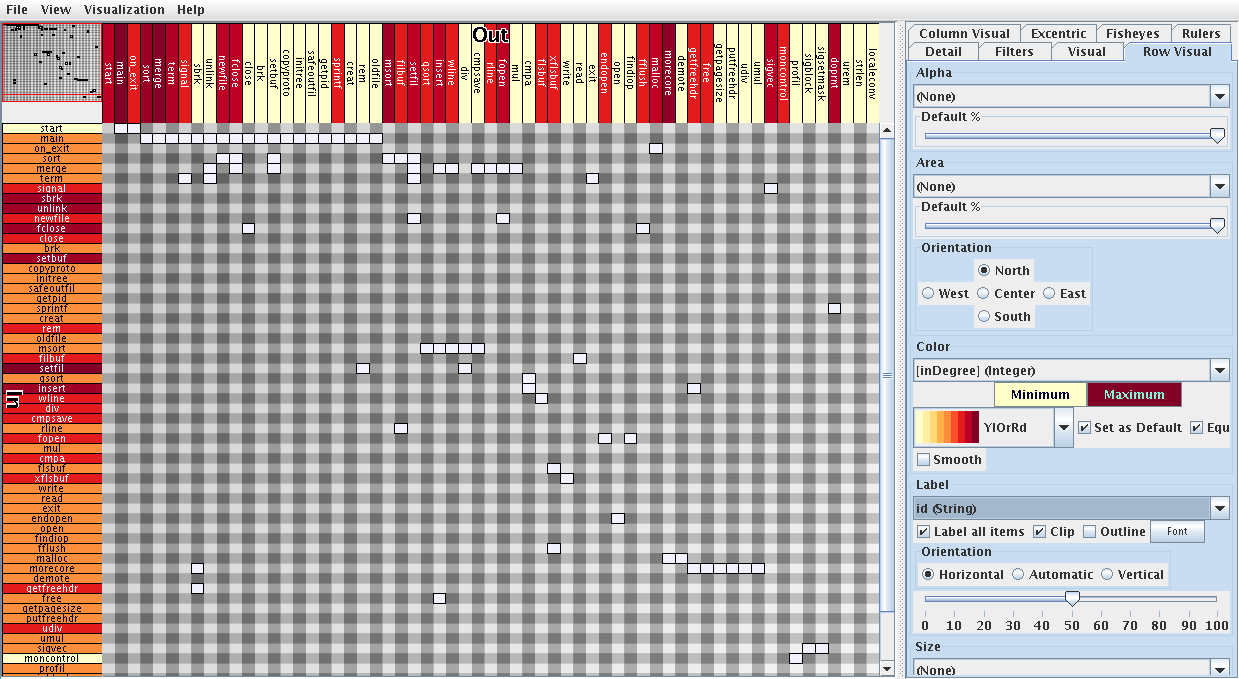
\includegraphics[keepaspectratio,width=\hsize,height=\halfh]
  {images/Header_MatrixExplorer_color.png}
  
  \caption[Matrix Header with Color Representation of Node Degree]{
  The intensity of the color in the node label represents the node degree.
  \imgcredit{Screenshot created by an author of this thesis using Matrix Explorer. \citep{henry-phd-2008}.}
  }
  \label{fig:header_matrixexplorer_color}
\end{figure}

\section{Histogram per Matrix Sub-Section}
In contrast to the histogram computed per node as explained in \ref{sec:histogram-per-node} , a histogram can also be computed over multiple columns or rows at the same time. Figure \ref{fig:header_matrixzoom_histogram} shows an example. The screenshot was taken from the matrix visualization program MatrixZoom. The displayed matrix is divided into three times three sub-sections. For every group of three vertically or horizontally aligned sections the amount of data contained in it is computed. Next, those values are transformed into a histogram representation, which is then drawn as light blue bars on the right and bottom matrix header. The result shows that the center section of the matrix has the largest density of data points of all sub-sections.

\begin{figure}[tp]
  \centering
  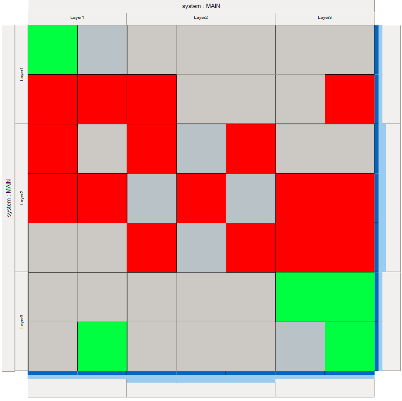
\includegraphics[keepaspectratio,width=\hsize,height=\halfh]
  {images/Header_MatrixZoom_histogram.png}
  \caption[Matrix Header with Histogram of Matrix Section Density]{
  The matrix is divided into nine different sub-sections. For each row and column of sub-sections the density of data points is computed. The result is drawn as light blue bars in the right and bottom matrix header.
  \imgcredit{Screenshot created by an author of this thesis using Matrix Zoom. \citep{ham2005phd}.}
  \label{fig:header_matrixzoom_histogram}}
\end{figure}
